\chapter{AHTR One-Third Assembly Optimization Results}
\glsresetall
\label{chap:ahtr-assem-opt-results}
In this chapter, I report the \gls{AHTR} one-third assembly's \gls{ROLLO} optimization 
results. 
I vary the following \gls{AHTR} one-third assembly input parameters:
\begin{itemize}
    \item \gls{TRISO} packing fraction distribution ($\rho_{TRISO}(\vec{r})$)
    \item Total fuel packing fraction ($PF_{total}$)
    \item \gls{FLiBe} coolant channel shape
\end{itemize} 
And, I optimize the \gls{AHTR} one-third assembly for the following optimization 
objectives:
\begin{itemize}
    \item Minimize total fuel packing fraction ($PF_{total}$)
    \item Minimize maximum one-third assembly temperature ($T_{max}$)
    \item Minimize fuel-normalized power peaking factor (PPF)
\end{itemize} 
 
In Chapter \ref{chap:method}, I detailed the methodology for \gls{AHTR} one-third 
assembly modeling and \gls{ROLLO} optimization. 
Section \ref{sec:ahtr-assem-geometry} describes the \gls{AHTR} one-third assembly 
geometry.
Section \ref{sec:input-parameter-modeling} details about how I vary the 
\gls{AHTR} one-third assembly's input parameters. 
Sections \ref{sec:ahtr-moltres-hom} and \ref{sec:ahtr_model_verification}
describe and verify the \gls{AHTR} one-third assembly's OpenMC neutronics and Moltres 
temperature models. 
Section \ref{sec:opt-problem} describes the optimization objectives and Section 
\ref{sec:ahtr_slab_output} describes how I calculated them from the OpenMC and Moltres 
model outputs. 
Section \ref{sec:hyperparameter-studies} describes the hyperparameter tuning process 
to select hyperparameters for the single-objective and multi-objective \gls{ROLLO} 
optimization simulations.

The subsequent sections outline the \gls{AHTR} one-third assembly's optimization 
simulations, describe the results of the single-objective and multi-objective 
\gls{ROLLO} optimization simulations, report each simulation's computational cost, 
and discuss the results' significance.

\section{ROLLO AHTR One-Third Assembly Optimization Simulations Overview}
Table \ref{tab:assem-obj-breakdown} shows the details of each \gls{ROLLO} 
optimization problems explored in this chapter.
\begin{table}[htbp]
    \centering
    \onehalfspacing
    \caption{\acrfull{ROLLO} simulations for optimizing \acrfull{AHTR}
    one-third assembly. $PF_{total}$: Total Fuel Packing Fraction, 
    $T_{max}$: Maximum one-third assembly Temperature, 
    $PPF$: Normalized Power Peaking Factor, $\rho_{TRISO}(\vec{r})$: 
    \gls{TRISO} packing fraction distribution}
	\label{tab:assem-obj-breakdown}
    \footnotesize
    \begin{tabular}{p{1.4cm}|p{1cm}|llll}
    \hline 
    \textbf{Num of Objs} & \textbf{Sim} & \textbf{Objectives} & \textbf{Constraints} &\textbf{Varying Parameters} & \textbf{Simulation Software} \\
    \hline
    \multirow{9}{2cm}{1}& a-1a & \tabitem min($PF_{total}$) & \tabitem $k_{eff}$ $>$ 1.0 &\tabitem $\rho_{TRISO}(\vec{r})$ & OpenMC \\
    & & & & \tabitem $PF_{total}$ & \\
    \cline{2-6}
    & a-1b & \tabitem min($T_{max}$) & \tabitem $k_{eff}$ $>$ 1.0 &\tabitem $\rho_{TRISO}(\vec{r})$ & OpenMC, Moltres\\
    \cline{2-6}
    & a-1c & \tabitem min($PPF$) & \tabitem $k_{eff}$ $>$ 1.0 &\tabitem $\rho_{TRISO}(\vec{r})$ & OpenMC\\
    \cline{2-6}
    & a-1d & \tabitem min($PF_{total}$) & \tabitem $k_{eff}$ $>$ 1.0 &\tabitem FLiBe channel shape & OpenMC \\
    & & & & \tabitem $PF_{total}$ & \\
    \cline{2-6}
    & a-1e & \tabitem min($T_{max}$) & \tabitem $k_{eff}$ $>$ 1.0 &\tabitem FLiBe channel shape & OpenMC, Moltres\\
    \cline{2-6}
    & a-1f & \tabitem min($PPF$) & \tabitem $k_{eff}$ $>$ 1.0 &\tabitem FLiBe channel shape & OpenMC\\
    \hline
    \multirow{6}{2cm}{2}& a-2a & \tabitem min($PF_{total}$) & \tabitem $k_{eff}$ $>$ 1.0 & \tabitem $\rho_{TRISO}(\vec{r})$ & OpenMC, Moltres\\
    & &\tabitem min($T_{max}$) & & \tabitem $PF_{total}$ & \\
    \cline{2-6}
    & a-2b & \tabitem min($PF_{total}$) & \tabitem $k_{eff}$ $>$ 1.0 & \tabitem $\rho_{TRISO}(\vec{r})$ & OpenMC\\
    & & \tabitem min($PPF$) & & \tabitem $PF_{total}$ & \\
    \cline{2-6}
    & a-2c & \tabitem min($T_{max}$) & \tabitem $k_{eff}$ $>$ 1.0 & \tabitem $\rho_{TRISO}(\vec{r})$ & OpenMC, Moltres\\
    & & \tabitem min($PPF$) & & & \\
    \hline
    \multirow{6}{2cm}{3}& a-3a &\tabitem min($PF_{total}$) & \tabitem $k_{eff}$ $>$ 1.0 & \tabitem $\rho_{TRISO}(\vec{r})$ & OpenMC, Moltres\\
    && \tabitem min($PPF$) & & \tabitem $PF_{total}$ & \\
    && \tabitem min($T_{max}$) & & & \\
    \cline{2-6}
    & a-3b &\tabitem min($PF_{total}$) & \tabitem $k_{eff}$ $>$ 1.0 & \tabitem $\rho_{TRISO}(\vec{r})$ & OpenMC, Moltres\\
    && \tabitem min($PPF$) & & \tabitem $PF_{total}$ & \\
    && \tabitem min($T_{max}$) & & \tabitem FLiBe channel shape& \\
    \hline
    \end{tabular}
\end{table}
I first conducted single objective, single input parameter \gls{ROLLO} optimizations 
to understand the individual impacts of each objective on each input parameter. 
Their results will inform the multi-objective optimization simulations setup. 

Simulations are run on the BlueWaters supercomputer \cite{ncsa_about_2017} and Theta 
supercomputer at the Argonne Leadership Computing Facility under the Director's 
Discretionary Allocation Program \cite{noauthor_argonne_2022}. 
Section \ref{sec:assem-compute-cost} details each optimization simulation's computational 
cost.  

\section{AHTR One-Third Assembly: Single-Objective Optimization Results}

\subsection{Objective: Minimize Total Packing Fraction}
\subsubsection{Simulation a-1a: Variation of $\rho_{TRISO}(\vec{r})$ and $PF_{total}$}
Table \ref{tab:simulationa1a} shows simulation a-1a's optimization problem parameters. 
\begin{table}[htbp]
    \centering
    \onehalfspacing
    \caption{Simulation a-1a Optimization Problem Parameters}
	\label{tab:simulationa1a}
    \footnotesize
    \begin{tabular}{l|p{3cm}}
    \hline 
    \multicolumn{2}{c}{\textbf{Single Objective: Simulation a-1a}} \\
    \hline 
    \textbf{Objectives} & Minimize $PF_{total}$ \\
    \hline 
    \textbf{Input Parameter variations} & $0.02<PF_{total}<0.04$ \\
    & $0<a<2$, $0<d<2$\\
    & $0<b<\frac{\pi}{2}$, $0<e<\frac{\pi}{2}$\\
    & $0<c<2\pi$, $0<f<2\pi$\\
    \hline
    \textbf{Constraints} & $k_{eff} > 1.0$\\ 
    \hline 
    \textbf{Genetic Algorithm Parameters} & Population size: 128 \\
    & Generations: 3 \\
    \hline
    \end{tabular}
\end{table}
Figure \ref{fig:assem-obj-1-pf-evol} shows the total packing fraction evolution and 
Figure \ref{fig:assem-obj-1-pf-final} shows the four TRISO packing fraction distributions in 
the final generation with the most minimized packing fractions. 
\begin{figure}[htbp]
    \centering
    \begin{subfigure}{\textwidth}
        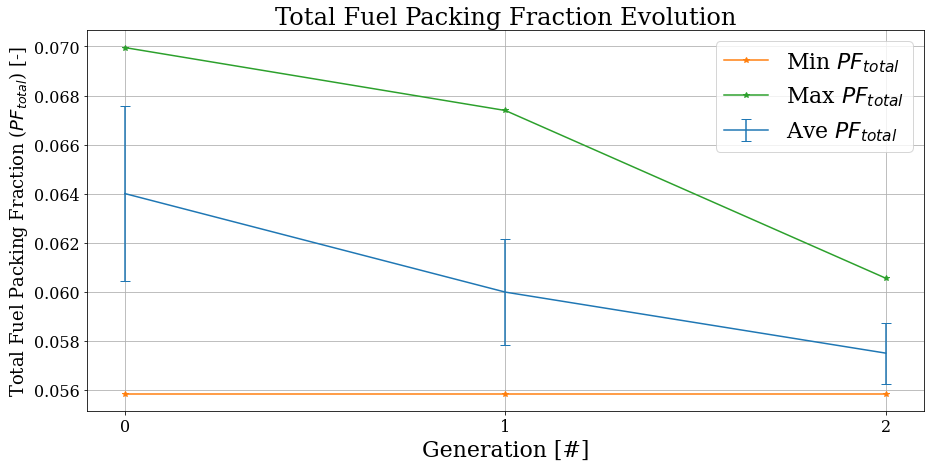
\includegraphics[width=\linewidth]{assem-obj-1-pf-evol.png}
        \caption{Minimum, average, and maximum total packing fraction evolution.}
        \label{fig:assem-obj-1-pf-evol} 
    \end{subfigure}
    \begin{subfigure}{\textwidth}
        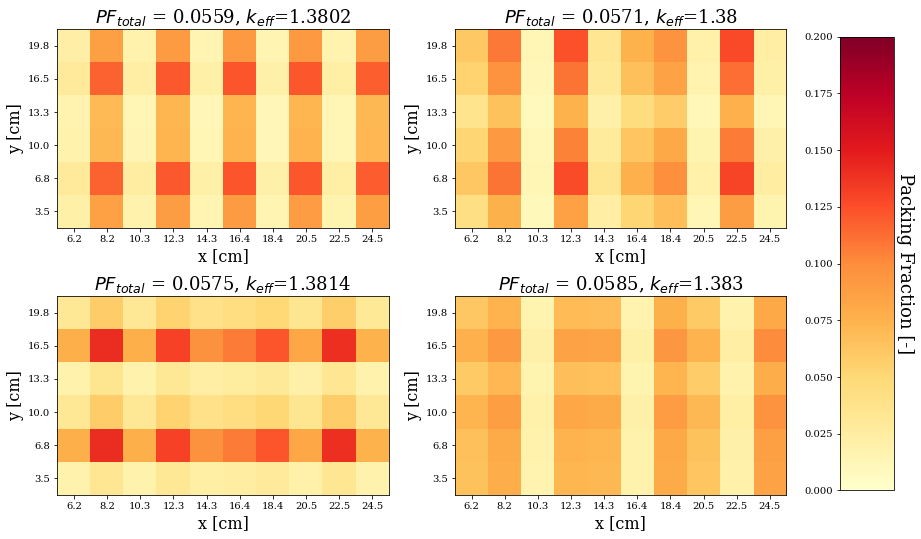
\includegraphics[width=\linewidth]{assem-obj-1-pf-final.png}
        \caption{TRISO packing fraction distribution for the 4 individuals with the 
        smallest packing fraction in generation 3.}
        \label{fig:assem-obj-1-pf-final} 
    \end{subfigure}
    \caption{ROLLO single-objective optimization to minimize total packing fraction. 
    Input parameters varied: total packing fraction, TRISO packing fraction distribution.}
    \label{fig:assem-obj-1-pf}
\end{figure}
The minimum and average packing fractions converged very quickly, as expected 
in this single-objective optimization problem.
By the $3^{rd}$ generation, the average and minimum packing fraction
values converged to approximately 0.017. 
In Figure \ref{fig:assem-obj-1-pf-final}, the four TRISO packing fraction distributions in the
final generation that minimized total packing fraction are the same.
The TRISO packing fraction peaks in the center of the assembly and is lower at the sides. 
By minimizing the packing fraction at the sides, the assembly minimizes self-shielding effects, 
enabling a lower packing fraction for the same $k_{eff}$. 

\subsection{Objective: Minimize Maximum Temperature ($T_{max}$)}

\subsection{Objective: Minimize Fuel-Normalized Power Peaking Factor (PPF)}
\subsubsection{Simulation a-1c: Variation of $\rho_{TRISO}(\vec{r})$}
Table \ref{tab:simulationa1c} shows simulation a-1c's optimization problem parameters. 
\begin{table}[htbp]
    \centering
    \onehalfspacing
    \caption{Simulation a-1c Optimization Problem Parameters}
	\label{tab:simulationa1c}
    \footnotesize
    \begin{tabular}{l|p{3cm}}
    \hline 
    \multicolumn{2}{c}{\textbf{Single Objective: Simulation a-1c}} \\
    \hline 
    \textbf{Objectives} & Minimize PPF \\
    \hline 
    \textbf{Input Parameter variations}
    & $PF_{total}$ = 0.04 \\
    & $0<a<2$, $0<d<2$\\
    & $0<b<\frac{\pi}{2}$, $0<e<\frac{\pi}{2}$\\
    & $0<c<2\pi$, $0<f<2\pi$\\
    \hline
    \textbf{Constraints} & $k_{eff} > 1.0$\\ 
    \hline 
    \textbf{Genetic Algorithm Parameters} & Population size: 64 \\
    & Generations: 3 \\
    \hline
    \end{tabular}
\end{table}
Figure \ref{fig:assem-obj-1-ppf-evol} shows the normalized power peaking factor evolution 
and Figure \ref{fig:assem-obj-1-ppf-final} shows the four TRISO packing fraction distributions in 
the final generation with the most minimized PPF. 
\begin{figure}[htbp]
    \centering
    \begin{subfigure}{\textwidth}
        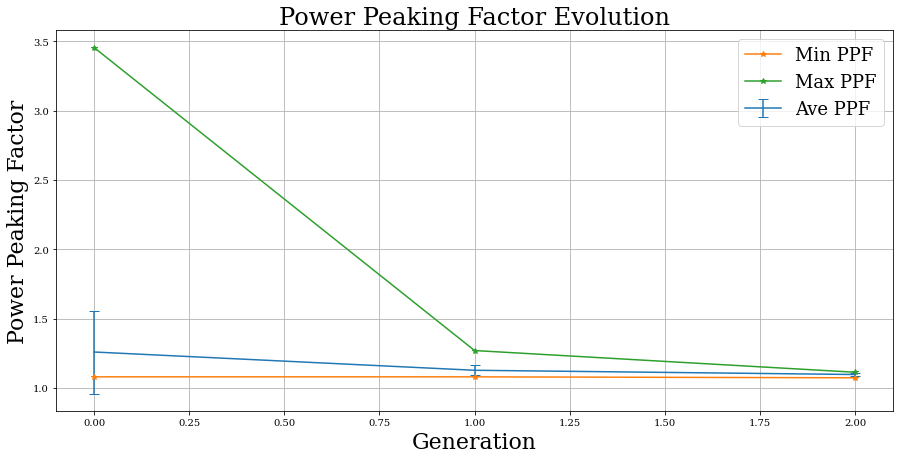
\includegraphics[width=\linewidth]{assem-obj-1-ppf-evol.png}
        \caption{Minimum, average, and maximum normalied power peaking factor evolution.}
        \label{fig:assem-obj-1-ppf-evol} 
    \end{subfigure}
    \begin{subfigure}{\textwidth}
        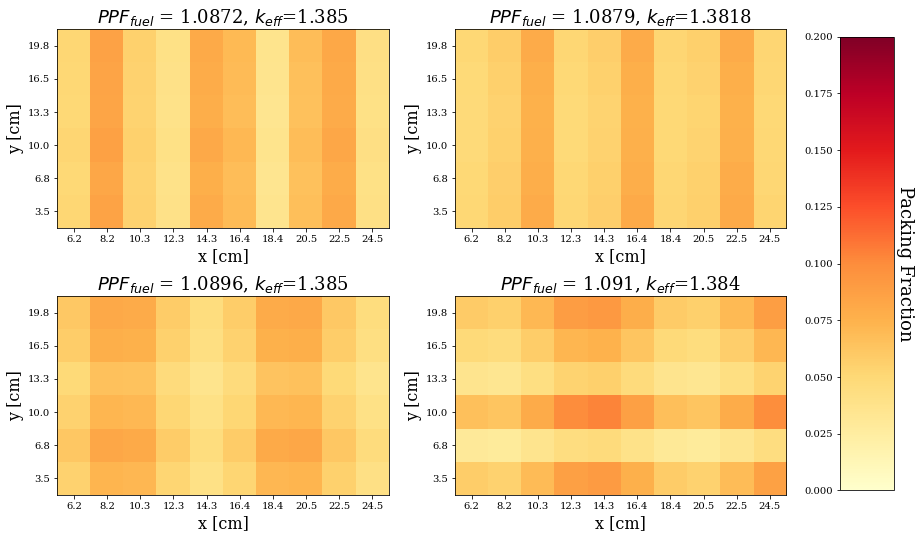
\includegraphics[width=\linewidth]{assem-obj-1-ppf-final.png}
        \caption{TRISO packing fraction distribution for the 4 individuals with the 
        smallest normalized power peaking factor in generation 3.}
        \label{fig:assem-obj-1-ppf-final} 
    \end{subfigure}
    \caption{ROLLO single-objective optimization to minimize total packing fraction. 
    Input parameters varied: total packing fraction, TRISO packing fraction distribution.}
    \label{fig:assem-obj-1-ppf}
\end{figure}

\section{AHTR One-Third Assembly: Two-Objective Optimization Results}

\section{AHTR One-Third Assembly: Three-Objective Optimization Results}

\section{AHTR One-Third Assembly: Computational Cost Summary}
\label{sec:assem-compute-cost}
Optimization simulations are run on the Theta supercomputer at the Argonne Leadership 
Computing Facility under the Director's Discretionary Allocation Program 
\cite{noauthor_argonne_2022}. 
Each Theta compute node has 64 processor cores with a nominal clock speed of 
1.5GHz \cite{noauthor_argonne_2022}.  

Each optimization simulation takes a different amount of node-hours to run due to 
differences in simulation software, tallies and intermediate steps required. 
Table \ref{tab:assem-compute-cost} reports the computational cost for each optimization 
simulation. 
Table \ref{tab:assem-obj-breakdown} detailed the simulation parameters.
\begin{table}[htbp!]
    \centering
    \onehalfspacing
    \caption{Computational cost of \acrfull{ROLLO} simulations for optimizing 
    \acrfull{AHTR} one-third assembly. BW: BlueWaters Supercomputer, Theta: Theta 
    supercomputer.}
	\label{tab:assem-compute-cost}
    \footnotesize
    \begin{tabular}{p{1.4cm}|p{1cm}lp{4cm}lp{4cm}}
    \hline 
    \textbf{Num of Objs} & \textbf{Sim} & \textbf{Machine} & 
    \textbf{Compute cost per gen [node-hours]} &\textbf{gens} & 
    \textbf{Total compute cost [node-hours]} \\
    \hline
    \multirow{6}{2cm}{1} 
    & a-1a & Theta &  &  &  \\
    & a-1b & Theta &  &  &  \\
    & a-1c & Theta &  &  &  \\
    & a-1d & Theta &  &  &  \\
    & a-1e & Theta &  &  &  \\
    & a-1f & Theta &  &  &  \\
    \hline
    \multirow{3}{2cm}{2}
    & a-2a & Theta &  &  &  \\
    & a-2b & Theta &  &  &  \\
    & a-2c & Theta &  &  &  \\
    \hline
    \multirow{2}{2cm}{3}
    & a-3a & Theta &  &  &  \\
    & a-3b & Theta &  &  &  \\
    \hline
    \end{tabular}
\end{table}

\section{AHTR One-Third Assembly Optimization Results Discussion and Significance}
\label{sec:assem-discussion}